\chapter{Własne propozycje rozwiązań}
    \section{Pozyskanie i agregowanie danych} \label{data_aggregation}
        \subsection{Europejska baza danych piłkarskich}
        \subsection{Elo Rating klubów piłkarskich}
        \subsection{Historyczne dane zakładów piłkarskich}
        \subsection{Metody agregacji}
    \section{Web API}
    \section{Wizualizacja charakterystyk danych}
    \noindent Przed przystąpieniem do właściwego przetwarzania danych i tworzenia na ich podstawie cech, warto bliżej im się przyjrzeć w celu potwierdzenia ich prawidłowości i wyszukania potencjalnych błędów i braków. Ten podrozdział poświęcony jest wizualizacji charakterystyk danych, które posiadamy w naszej bazie. Wizualizacja została dokonana w \emph{Jupyter Notebook}, a jej plik źródłowy znajduje się w repozytorium projektu~\cite{repo} w folderze \texttt{visualization/} pod nazwą \texttt{visualization.ipynb}
    
    Podczas wizualizacji pomijane są tabele, które są z jej punktu widzenia mało istotne - tabelę \emph{Team} (ponieważ zawiera ona tylko nazwy drużyn) i tabele \emph{Country} oraz \emph{League} (posiadają one tylko jeden wiersz - analizujemy rozgrywki z jednego kraju oraz jednej ligi). Podobnie z atrybutami - pomijane będą klucze podstawowe oraz klucze obce.
    
    ~
    
    Pierwszą tabelą wartą głębszej analizy jest tabela \emph{Team\_Attributes}. Zawiera ona pewne statystyki dla każdej z drużyn. Oto jak prezentuje się zestawienie kolumn tej tabeli wraz z ich typami i liczbą wartości niepustych:
    
    \begin{table}[H]
    \caption{Kolumny tabeli Team\_Attributes}
    \centering\footnotesize%
    \begin{tabular}{l c c}
    \toprule
        Nazwa & Liczba niepustych wartości & Typ \\
    \midrule
        date & 204 & datetime64 \\
        buildUpPlaySpeed & 204 & int64 \\
        buildUpPlaySpeedClass & 204 & int64 \\
        buildUpPlayDribbling & 68 & float64 \\
        buildUpPlayDribblingClass & 204 & string \\
        buildUpPlayPassing & 204 & float64 \\
        buildUpPlayPassingClass & 204 & string \\
        buildUpPlayPositioningClass & 204 & string \\
        chanceCreationPassing & 204 & int64 \\
        chanceCreationPassingClass & 204 & string \\
        chanceCreationCrossing & 204 & int64 \\ 
        chanceCreationCrossingClass & 204 & string \\        
        chanceCreationShooting & 204 & int64 \\  
        chanceCreationShootingClass & 204 & string \\
        chanceCreationPositioningClass & 204 & string \\
        defencePressure & 204 & int64 \\
        defencePressureClass & 204 & string \\
        defenceAggression & 204 & int64 \\  
        defenceAggressionClass & 204 & string \\
        defenceTeamWidth & 204 & int64 \\
        defenceTeamWidthClass & 204 & string \\
        defenceDefenderLineClass & 204 & string \\
    \bottomrule
    \end{tabular}
    \end{table}
    
    \noindent Wszystkich wierszy w tabeli jest 204, stąd na powyższym zestawieniu widać, że jedynym atrybutem, który nie ma uzupełnionych wartości dla wszystkich rekordów jest \emph{buildUpPlayDribbling}. Z uwagi na to, że brakujących wartości jest dosyć dużo (prawie 70\% wierszy w tabeli nie ma podanej wartości dla tego atrybutu), zdecydowano się go nie uwzględniać przy dalszym przetwarzaniu. Pomijane są również wszystkie kolumny typu \emph{string}, ponieważ są one tylko kategoriami (klasami) dla odpowiadających im wartości numerycznych.
    
    Warto również przyjrzeć się histogramom wszystkich atrybutów numerycznych w celu weryfikacji poprawności ich zakresów.
    
    \begin{figure}[H] 
        \centering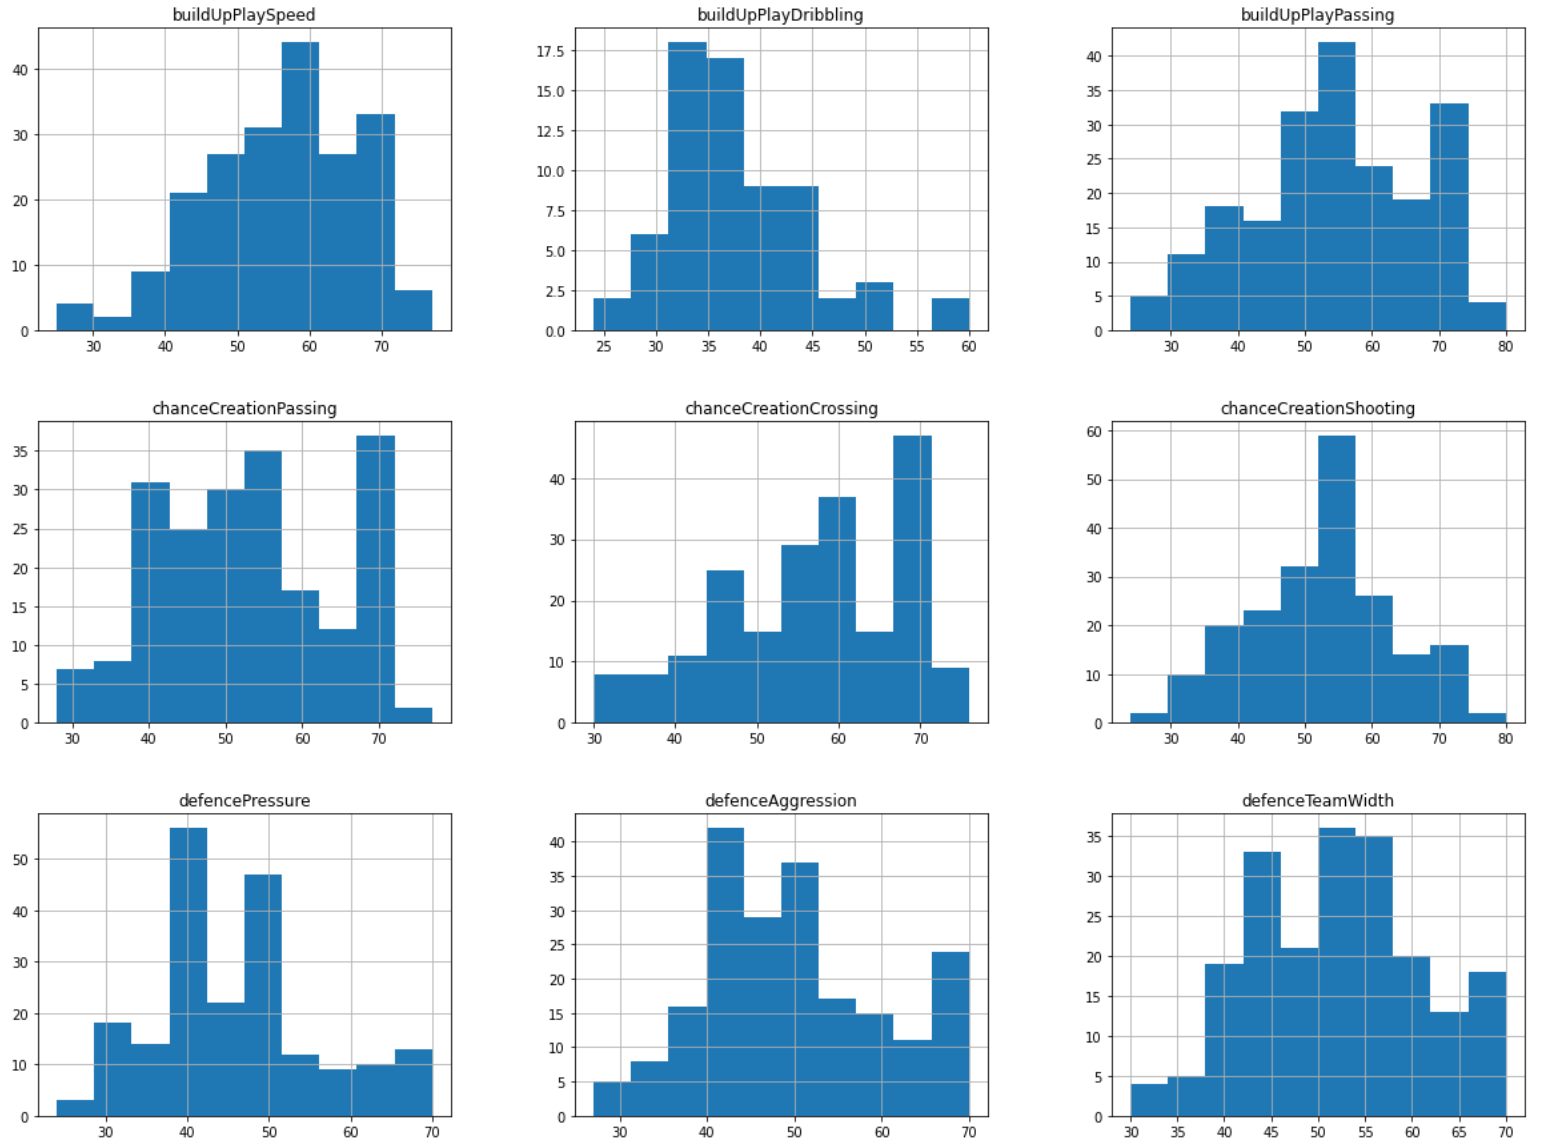
\includegraphics[width=\textwidth]{figures/team_attributes.png}
        \caption{Histogramy wartości numerycznych tabeli Team\_Attributes}
        \label{fig:team_attributes}
    \end{figure}
    
    \noindent Jak można zaobserwować na rysunku~\ref{fig:team_attributes}, wszystkie atrybuty mają odpowiednie zakresy - nie ma wartości odstających, wszystkie są dodatnie. W ich przypadku dalsze przetwarzanie nie będzie konieczne.\\*
    
    \noindent Kolejną analizowaną tabelą jest tabela \emph{Player}. Posiada ona podstawowe informacje o wszystkich graczach.
    
    \begin{table}[H]
    \caption{Kolumny tabeli \emph{Player}}\label{tab:player}
    \centering\footnotesize%
    \begin{tabular}{l c c}
    \toprule
        Nazwa & Liczba niepustych wartości & Typ \\
    \midrule
        player\_name & 1397 & string \\
        birthday & 1397 & datetime64 \\
        height & 1397 & int64 \\
        weight & 1397 & int64 \\
    \bottomrule
    \end{tabular}
    \end{table}
    
    \noindent Wszystkich wierszy w tabeli Player jest 1397. Zgodnie z tablicą~\ref{tab:player}, tabela nie posiada wartości pustych. Z uwagi na trudność wizualizacji atrybutu \emph{birthday}, wprowadzony zostanie nowy, sztuczny atrybut wieku (\english{age}), który pozwoli zweryfikować jego poprawność. \\*
    
    \begin{figure}[H] 
        \centering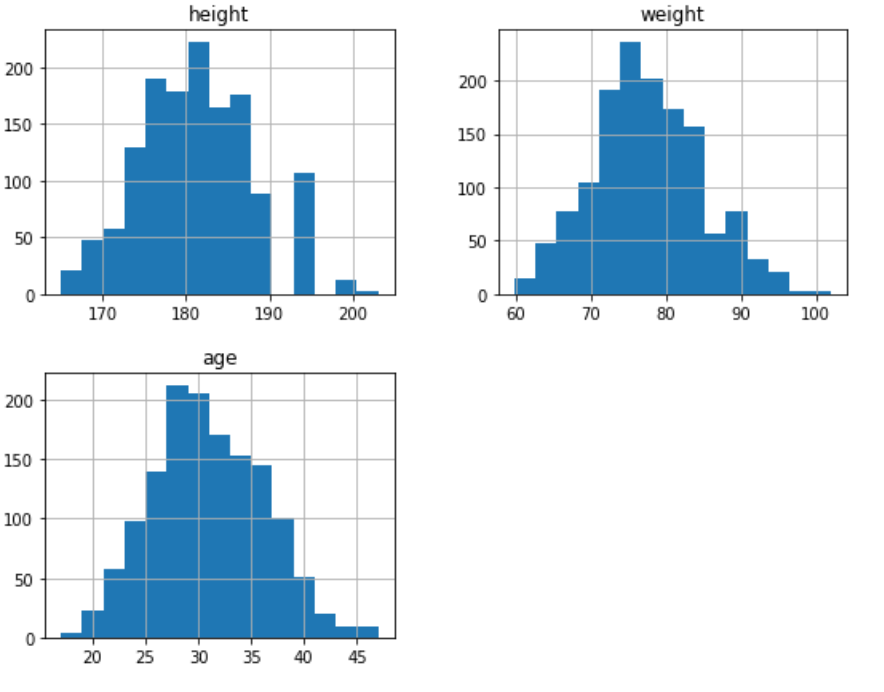
\includegraphics[width=\textwidth]{figures/player.png}
        \caption{Histogramy wartości dla atrybutów tabeli \emph{Player}}
        \label{fig:player}
    \end{figure}
    
    \noindent Spoglądając na rysunek~\ref{fig:player} zauważamy, że rozkłady wartości wszystkich atrybutów przypominają rozkłady normalne. Tutaj podobnie jak w przypadku poprzedniej tabeli, zakresy są poprawne. Warto zaznaczyć, że waga (\english{weight}) na potrzeby wizualizacji została przedstawiona w kilogramach, a wysokość (\english{height}) w centymetrach. Omówiony wcześniej sztuczny atrybut wieku pozwolił zweryfikować prawidłowość wartości dla kolumny \textit{birthday}. \\*
    
    \noindent Inną tabelą związaną z graczami jest tabela \emph{Player\_Attributes}. Zawiera ona pewne statystyki odnośnie każdego z graczy dotyczące jego umiejętności. Przyglądając się schematowi naszej bazy danych na rysunku~\ref{database_schema}, można zaobserwować, że tabela ta posiada dużo różnych atrybutów numerycznych. Istotne jednak z punktu widzenia późniejszego tworzenia cech jest istnienie atrybutu zwanego \emph{overall\_rating}, który można na język polski przetłumaczyć jako ,,ogólna ocena''. Jest on pewną agregacją wszystkich pozostałych atrybutów dokonaną przez twórców gry Fifa. Dzięki niemu można pominąć pozostałe atrybuty i do dalszego przetwarzania uwzględnić wyłącznie ten.
    
    \begin{figure}[H] 
        \centering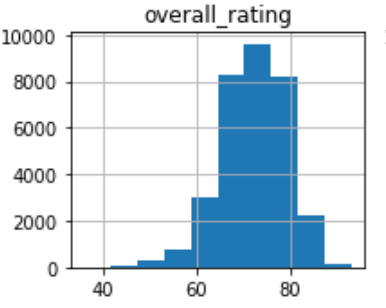
\includegraphics[width=5cm]{figures/overall_rating.png}
        \caption{Histogram wartości atrybutu \emph{overall\_rating}}
        \label{fig:overall_rating}
    \end{figure}
    
    \noindent Dodatkowym jego atutem (co można zauważyć na rysunku~\ref{fig:overall_rating}) jest poprawność zakresu jego wartości oraz fakt, że jest on zdefiniowany dla każdego gracza w bazie danych.
    
    Atrybuty kategoryczne, m.in \emph{preferred foot} (,,preferowana noga''), zostały pominięte ze względu na wątpliwy wpływ na predykcję wyniku meczu. \\*
    
    \noindent \emph{EloRating} jest tabelą, która zawiera wartości tzw. atrybutu \emph{Elo} aktualnego na dany dzień dla każdej z drużyn.
    
    \begin{table}[H]
    \caption{Kolumny tabeli EloRating}\label{tab:elo}
    \centering\footnotesize%
    \begin{tabular}{l c c}
    \toprule
        Nazwa & Liczba niepustych wartości & Typ \\
    \midrule
        team\_name & 31607 & string \\
        rank & 31607 & int64 \\
        Elo & 31607 & float64 \\
        start\_date & 31607 & datetime64 \\
        end\_date & 31607 & datetime64 \\
    \bottomrule
    \end{tabular}
    \end{table}
    
    \begin{table}[H]
    \caption{Przykładowe rekordy w tabeli EloRating}\label{tab:elo_example}
    \centering\footnotesize%
    \begin{tabular}{l c c c c}
    \toprule
        team\_name & rank & Elo & start\_date & end\_date \\
    \midrule
        Manchester United & 14 & 1843.027344 & 2014-08-17 & 2014-08-19\\
        Manchester United & 14 & 1842.388550 & 2014-08-20 & 2014-08-21\\
        Manchester United & 15 & 1840.082642 & 2014-08-22 & 2014-08-23\\
        Manchester United & 14 & 1840.082642 & 2014-08-24 & 2014-08-24\\
        Manchester United & 14 & 1836.078979 & 2014-08-25 & 2014-08-27\\
        Manchester United & 15 & 1837.623047 & 2014-08-28 & 2014-08-28\\
    \bottomrule
    \end{tabular}
    \end{table}
    
    \noindent Tablica~\ref{tab:elo} stanowi potwierdzenie uzupełnionych wartości atrybutów dla każdego rekordu w tabeli, a tablica~\ref{tab:elo_example} obrazuje, że dla każdej drużyny w naszej bazie może istnieć wiele rekordów. Każdy zawiera inną wartość atrybutu \emph{Elo} (wraz z miejscem zajmowanym w globalnym rankingu drużyn) aktualnym w danym przedziale czasowym. Atrybut ten ulega przeliczeniu po każdym rozegranym przez drużynę meczu.
    
    Tworząc wektory cech reprezentujące pojedynczy mecz, dla obu drużyn korzystamy z wartości tego atrybutu aktualnego na dzień meczu. Obrazuje on aktualną ,,formę'' drużyny w dniu rozgrywania meczu. \\*
    
    \noindent Najobszerniejszą tabelą w naszym systemie jest tabela \emph{Matches}. Każdy jej rekord reprezentuje jeden mecz pomiędzy dwoma drużynami wraz z jego charakterystykami, np. liczba strzałów drużyny gospodarzy, liczba żółtych kartek drużyny gości, kursy oferowane na remis itd.
    
    Z uwagi na sporą liczbę atrybutów w tej tabeli, warto ją podzielić na mniejsze części w celu łatwiejszej i czytelniejszej analizy. Pierwszą badanym zestawem są atrybuty związane z kursami od różnych zakładów bukmacherskich.
    
    \begin{table}[H]
    \caption{Podstawowe statystyki dla atrybutów związanych z kursami.}\label{tab:odds}
    \centering\footnotesize%
    \begin{tabular}{l c c c c c}
    \toprule
        Atrybut & \emph{count} & \emph{mean} & \emph{std} & \emph{min} & \emph{max} \\
    \midrule
        B365H & 3040 & 2.701964 & 1.689834 & 1.100000 & 15.000000\\
        BWH & 3039 & 2.603906 & 1.528913 & 1.100000 & 12.500000\\
        IWH & 3038 & 2.513644 & 1.368492 & 1.050000 & 10.000000\\
        LBH & 3039 & 2.611787 & 1.526034 & 1.080000 & 12.000000\\
        PSH & 1519 & 2.720369 & 1.575303 & 1.130000 & 10.800000\\
        WHH & 3040 & 2.663760 & 1.590124 & 1.100000 & 12.000000\\
        SJH & 2320 & 2.667828 & 1.698067 & 1.110000 & 15.000000\\
        VCH & 3040 & 2.712204 & 1.692001 & 1.090000 & 15.000000\\
        GBH & 1899 & 2.606840 & 1.586001 & 1.100000 & 12.000000\\
        BSH & 1900 & 2.625553 & 1.655792 & 1.100000 & 13.000000\\\\
        
        B365D & 3040 & 3.952720 & 0.998305 & 3.000000 & 11.000000\\
        BWD & 3039 & 3.803251 & 0.882597 & 2.900000 & 9.250000\\
        IWD & 3038 & 3.687903 & 0.735121 & 3.000000 & 10.000000\\
        LBD & 3039 & 3.815271 & 0.876612 & 2.880000 & 10.000000\\
        PSD & 1519 & 4.078183 & 1.046468 & 3.040000 & 11.030000\\
        WHD & 3040 & 3.669260 & 0.812509 & 2.800000 & 9.500000\\
        SJD & 2320 & 3.881039 & 0.926573 & 3.000000 & 9.000000\\
        VCD & 3040 & 3.955470 & 1.009081 & 2.500000 & 10.000000\\
        GBD & 1899 & 3.761980 & 0.842088 & 3.000000 & 8.500000\\
        BSD & 1900 & 0.837965 & 0.837965 & 3.000000 & 8.500000\\\\
        
        B365A & 3040 & 4.910437 & 3.909392 & 1.220000 & 29.000000\\
        BWA & 3039 & 4.495166 & 3.213833 & 1.220000 & 21.000000\\
        IWA & 3038 & 4.245671 & 2.919038 & 1.270000 & 25.000000\\
        LBA & 3039 & 4.563537 & 3.371435 & 1.220000 & 26.000000\\
        PSA & 1519 & 4.923970 & 3.840303 & 1.370000 & 28.500000\\
        WHA & 3040 & 4.699592 & 3.628486 & 1.220000 & 26.000000\\
        SJA & 2320 & 4.859233 & 3.826951 & 1.250000 & 29.000000\\
        VCA & 3040 & 4.956711 & 3.984335 & 1.220000 & 29.000000\\
        GBA & 1899 & 4.566435 & 3.301710 & 1.250000 & 21.000000\\
        BSA & 1900 & 3.786069 & 3.786069 & 1.220000 & 26.000000\\
    \bottomrule
    \end{tabular}
    \end{table}
    
    \noindent Tablica~\ref{tab:odds} zawiera pogrupowane kursy od różnych bukmacherów według zdarzeń. Ostatnia litera w nazwie atrybutu informuje o typie zdarzenia, na który jest oferowany ten kurs. Litera ,,H'' oznacza kurs oferowany na zwycięstwo drużyny gospodarzy, ,,D'' na remis, natomiast ,,A'' na zwycięstwo gości. Pozostałe litery tworzą skrót od nazwy danego bukmachera. Prezentowane statystyki to liczność (\english{count}) średnia (\english{mean}), odchylenie standardowe (\english{standard deviaton, std}), wartość minimalna oraz maksymalna.
    
    Jak można spostrzec analizując wartości średnie dla poszczególnych grup, na zwycięstwo gospodarzy oferowany jest średnio mniejszy kurs niż na pozostałe dwa zdarzenia. Pozwala to podejrzewać, że granie na swoim stadionie daje drużynie pewną przewagę. Potwierdza to fakt, że na zwycięstwo gości średnio ten kurs jest najwyższy.
    
    Warto również zwrócić uwagę na to, że w obrębie poszczególnych grup zdarzeń, średnie kursy proponowane przez bukmacherów są bardzo do siebie zbliżone. Oznacza to, że najprawdopodobniej ich modele matematyczne wyznaczają podobne prawdopodobieństwa dla danych zdarzeń. Dodatkowym istotnym faktem jest to, że dla każdej grupy zdarzeń istnieją przynajmniej dwa atrybuty, które są zdefiniowane dla każdego meczu (których liczność w naszej bazie danych wynosi 3400). Przykładowo, dla zdarzeń z grupy ,,zwycięstwo gospodarzy'' zawsze istnieje wartość dla atrybutu \emph{B365H} oraz \emph{WHH} (ich wartość \emph{count} wynosi 3400). Ten fakt, wraz z obserwacją o podobnych kursach w obrębie poszczególnych grup, umożliwiają poradzenie sobie z brakującymi wartościami niektórych atrybutów. Skoro wiadomo, że kursy na dane zdarzenie są podobne, wystarczy uwzględniać podczas późniejszego przetwarzania tylko te atrybuty, które mają wartość niepustą (mamy gwarancję obecności przynajmniej dwóch takich atrybutów dla każdego z trzech zdarzeń w meczu- zwycięstwa gospodarzy, remisu oraz zwycięstwa gości). \\*
    
    \noindent Kolejnym zestawem analizowanych atrybutów są te związane bezpośrednio z przebiegiem meczu. 
    
    \begin{table}[H]
    \caption{Wybrane atrybuty tabeli \emph{Matches}}\label{tab:matches}
    \centering\footnotesize%
    \begin{tabular}{l c c l}
    \toprule
        Nazwa & Liczba niepustych wartości & Typ & Wyjaśnienie \\
    \midrule
        HomeTeamShots & 3040 & int64 & liczba strzałów drużyny gospodarzy \\
        AwayTeamShots & 3040 & int64 & liczba strzałów drużyny gości \\
        HomeTeamShotsOnTarget & 3040 & int64 & liczba celnych strzałów drużyny gospodarzy \\
        AwayTeamShotsOnTarget & 3040 & int64 & liczba celnych strzałów drużyny gości \\
        HomeTeamCorners & 3040 & int64 & liczba rzutów rożnych drużyny gospodarzy \\
        AwayTeamCorners & 3040 & int64 & liczba rzutów rożnych drużyny gości \\
        HomeTeamFoulsCommitted & 3040 & int64 & liczba popełnionych fauli przez gospodarzy \\
        AwayTeamFoulsCommitted & 3040 & int64 & liczba popełnionych fauli przez gości \\
        HomeTeamYellowCards & 3040 & int64 & liczba żółtych kartek otrzymanych przez gospodarzy \\
        AwayTeamYellowCards & 3040 & int64 & liczba żółtych kartek otrzymanych przez gości \\
        AwayTeamRedCards & 3040 & int64 & liczba czerwonych kartek otrzymanych przez gości \\
        HomeTeamRedCards & 3040 & int64 & liczba żółtych kartek otrzymanych przez gospodarzy \\
    \bottomrule
    \end{tabular}
    \end{table}

     \begin{figure}[H] 
        \centering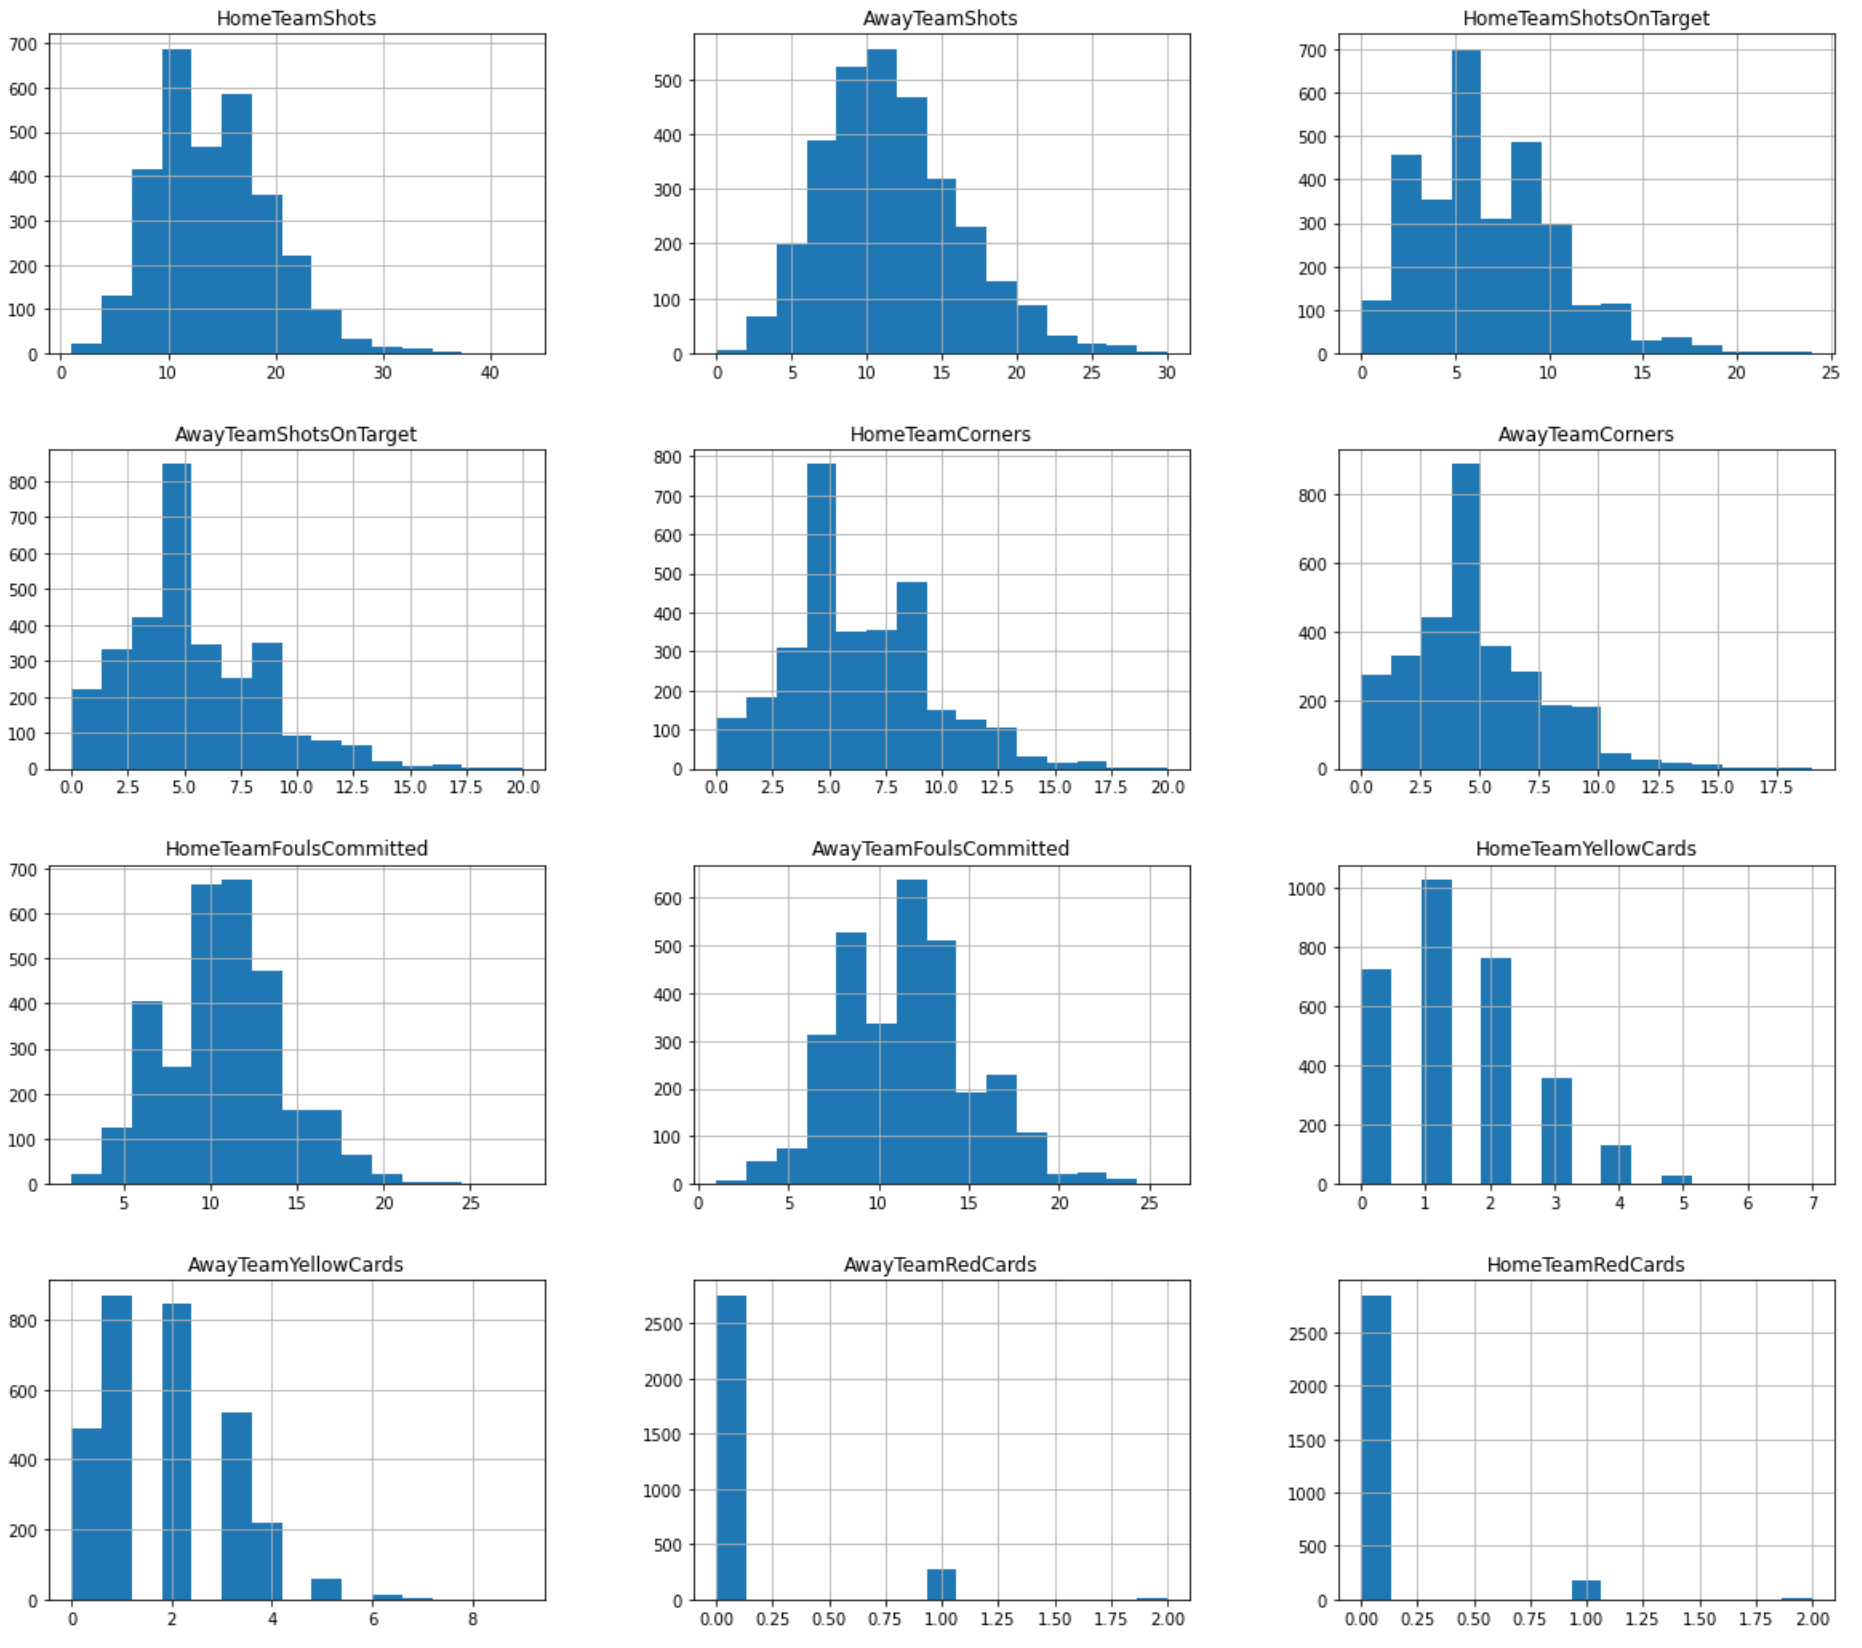
\includegraphics[width=\textwidth]{figures/matches.png}
        \caption{Histogramy wybranych atrybutów tabeli \emph{Matches}}
        \label{fig:matches}
    \end{figure}
    
    \noindent Tablica~\ref{tab:matches} utwierdza nas w przekonaniu, iż wszystkie atrybuty są uzupełnione i nie zawierają żadnych braków.
    Na rysunku~\ref{fig:matches} przedstawiono ich histogramy. Potwierdzają one zarówno poprawność ich zakresów, jak i pewne intuicyjne założenia, przykładowo - czerwone kartki są sporadycznym zdarzeniem i występują zdecydowanie rzadziej niż żółte kartki. 
    
    \section{Wstępne przetwarzanie}
    \noindent Na rysunku~\ref{fig:preprocessing_structure} przedstawiona została struktura modułu służącego do pobierania danych z serwera, ich wstępnego przetwarzania oraz tworzenia na ich podstawie cech. Moduł ten znajduje się w repozytorium projektu~\cite{repo} w folderze \texttt{Preprocessing/}.
    \begin{figure}[H] 
        \centering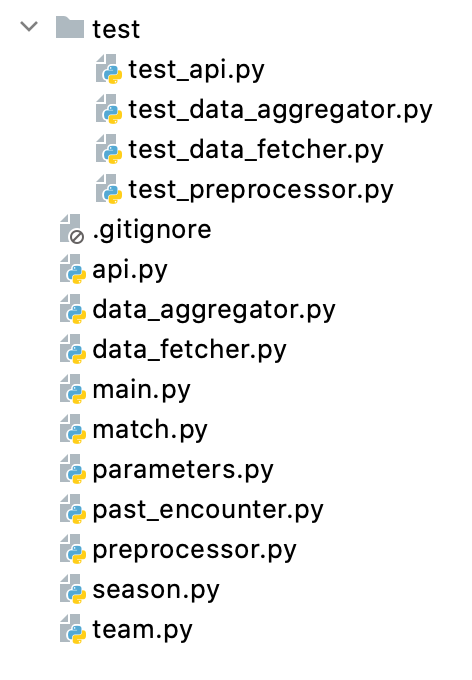
\includegraphics[width=6cm]{figures/preprocessing_structure.png}
        \caption{Struktura modułu do wstępnego przetwarzania}
        \label{fig:preprocessing_structure}
    \end{figure}
    
    Oprócz podfolderu \texttt{test/} (który zostanie szczegółowo omówiony w późniejszym podrozdziale), przechowującego wszystkie testy jednostkowe, znajdują się w nim też właściwe pliki odpowiedzialne za wspomniane funkcje modułu:
    
    \begin{itemize}
        \item \texttt{api.py}- plik zawierający funkcje pomocnicze do tworzenia odpowiedniego url'a, przy pomocy którego następuje wysłanie zapytanie do serwera,
        \item \texttt{data\_fetcher.py}- odpowiada za pobieranie danych z serwera przy użyciu \emph{WebApi},
        \item \texttt{data\_aggregator.py}- używa poprzedniego pliku w celu pobrania danych i służy do ich agregacji (np. danych dla kilku sezonów) w jeden zbiór danych; jest punktem wejściowym do biblioteki, który używa klient,
        \item \texttt{preprocessor.py}- przetwarza otrzymane dane i tworzy na ich podstawie wektory cech reprezentujące każdy mecz,
        \item \texttt{match.py}, \texttt{parameters.py}, \texttt{past\_encounters.py}, \texttt{season.py} oraz \texttt{team.py}- reprezentują modele danych używane w systemie i enkapsulują ich pewne właściwości (np. identyfikator dla sezonu lub drużyny, który jest potrzebny do wykonania zapytania do serwera),
        \item \texttt{main.py}- zawiera przykład użycia biblioteki.
    \end{itemize}
    
        \subsection{Pobieranie danych z serwera i ich agregacja}
        \noindent Moduł komunikuje się z serwerem przy pomocy udostępnionego przez niego interfejsu programistycznego. Komunikacja ta jest inicjowana przez klienta przy użyciu dwóch funkcji z pliku \texttt{data\_aggregator.py}:
        
        \begin{itemize}
            \item \texttt{get\_data\_for\_seasons()}
            \item \texttt{get\_data\_for\_team\_in\_seasons()}
        \end{itemize}
        
        Obie te funkcje przyjmują jako argument listę sezonów, dla których mają być pobrane dane oraz obiekt \emph{Parameters}, który pozwala sparametryzować zapytanie do serwera. Obiekt ten aktualnie posiada tylko jeden atrybut, który określa ile meczów z przeszłości dla danej drużyny brać pod uwagę przy pobieraniu danych.
        
        Dodatkowo, druga z funkcji pozwala na określenie drużyny, dla której mają być pobrane dane. Oto jak wygląda przykładowe wywołanie obu tych funkcji.
        
        \begin{lstlisting}[language=Python, label={lis:example_usage}, caption=Przykładowe wywołanie funkcji do pobrania danych]
        data_aggregator = DataAggregator()
        
        # pobierz dane dla sezonu 2011 i 2012
        data_aggregator.get_data_for_seasons([Season.y2011, Season.y2012], Parameters(no_last_matches=3))
        
        # pobierz dane dla Arsenalu z sezonu 2011 i 2012
        data_aggregator.get_data_for_team_in_seasons(Team.Arsenal, [Season.y2011, Season.y2012], Parameters(no_last_matches=3))
        \end{lstlisting}
        
        \noindent Zapytanie do serwera pozwala na pobranie danych jednorazowo dla konkretnego sezonu lub drużyny. Natomiast jak można zauważyć na listingu \ref{lis:example_usage}, klient ma możliwość wykonania zapytania dla kilku sezonów naraz. Tę możliwość udostępnia klasa \emph{DataAggregator}, która wewnętrznie wykonuje osobno zapytanie dla każdego sezonu i agreguje otrzymane dane w jeden zbiór, który zwracany jest klientowi.
        
        W celu pobrania danych, klasa \emph{DataAggregator} korzysta z klasy znajdujacęj się we wcześniej wspomnianym pliku \texttt{data\_fetcher.py} o nazwie \emph{DataFetcher}. Na listingu \ref{lis:data_fetcher} widać fragment tej klasy. Przy wykonywaniu zapytania, najpierw korzysta ona z funkcji pomocniczej do stworzenia odpowiedniego url'a, a później wykonuje faktyczne zapytanie i zwraca jego wynik. Warto również zwrócić uwagę na mechanizm z pamięcią podręczną. Po otrzymaniu odpowiedzi od serwera, jest ona zapisywana w pamięci pod odpowiednim kluczem. Przed wykonaniem zapytania do serwera, sprawdzane jest, czy nie zostało już wcześniej wykonane zapytanie z takimi samymi parametrami. Jeżeli tak, zwracany jest jego wynik.
        
        
        \begin{lstlisting}[language=Python, label={lis:data_fetcher}, caption=Fragment klasy \emph{DataFetcher}]
        class DataFetcher:

            def __init__(self):
                self.cache = {}

            def fetch_data_for_season(self, season, params):
                url = get_url_for_matches_in_season(season.value, params)
                if url in self.cache:
                    return self.cache[url]
                data = requests.get(url).text
                self.cache[url] = data
                return data
        \end{lstlisting}
    
        
        
        \subsection{Tworzenie zbioru cech (TBC)}
        \noindent Zbiór cech jest jednym z kluczowych czynników, które wpływają na jakość algorytmów uczenia maszynowego. Odpowiedni dobór oraz selekcja i segregacja to droga do uzyskania dobrej predykcji. Jednak wybór odpowiednich cech nie jest łatwym zadaniem i zazwyczaj zajmuje on dużo czasu i zasobów. Także w naszym problemie, dobór cech był starannie dokonany. Piłka nożna do bardzo rozbudowana gra i z jednej partii między drużynami można wyciągnąć nieskończoną ilość danych, poprzez najbardziej oczywiste jak liczba strzałów, po te mniej jak ilość minut spędzonych na swojej połowie przez danego gracza lub średni wiek piłkarza w danej drużynie. Z racji, że posiadaliśmy dość rozbudowaną bazę pochodzącą z różnych źródeł, ostatecznie wybraliśmy 30 cech, które odpowiednio zagregowaliśmy a następnie przekazaliśmy na wejście naszych algorytmów uczenia maszynowego. Lista tych cech wraz z ich krótkim wyjaśnieniem:
        
        \begin{itemize}
            \item \emph{avg\_away\_win\_odds}, \emph{avg\_home\_win\_odds}, \emph{avg\_draw\_odds}: średnia wartość kursów oferowanych na zwycięstwo danej drużyny, remis oraz wygraną drugiej drużyny,
            \item \emph{home\_elo\_rating}, \emph{away\_elo\_rating}: \emph{EloRating} dla obu drużyn,
            \item \emph{home\_players\_avg\_age}, \emph{away\_players\_avg\_age}: średni wiek graczy w drużynach, 
            \item \emph{home\_players\_avg\_rating}, \emph{away\_players\_avg\_rating}: średnia siła zawodników danej drużyny (statystyki z gry Fifa), 
            \item \emph{home\_team\_score}, \emph{away\_team\_score}: siła drużyn (statystyki z gry Fifa, takie jak: szybkość budowania ataku, ilość wymienianych podań...), 
            \item \emph{home\_avg\_corners}, \emph{away\_avg\_corners}: średnia liczba rzutów rożnych na mecz danej drużyny w ciągu ostatnich X meczów, 
            \item \emph{home\_avg\_shots}, \emph{away\_avg\_shots}: średnia liczba oddanych strzałów na mecz danej drużyny w ciągu ostatnich X meczów, 
            \item \emph{home\_won\_games}, \emph{away\_won\_games}: liczba wygranych przez drużynę spotkań z ostatnich X meczów, 
            \item \emph{home\_tied\_games}, \emph{away\_tied\_games}: liczba remisów w ostatnich X meczach, 
            \item \emph{home\_lost\_games}, \emph{away\_lost\_games}: liczba przegranych w ostatnich X meczach, 
            \item \emph{home\_scored\_goals}, \emph{away\_scored\_goals}: liczba strzelonych przez drużynę goli w ostatnich X meczach, 
            \item \emph{home\_team\_last\_season\_points}, \emph{away\_team\_last\_season\_points}: zdobyte punkty przez drużynę w ostatnim sezonie, 
            \item \emph{home\_team\_seasons\_played}, \emph{away\_team\_seasons\_played}: liczba sezonów, które dana drużyna gra w Premier League, 
            \item \emph{home\_direct\_wins}: liczba zwycięstw drużyny gospodarza nad drużyną gościa w ostatnich X meczach rozgrywanych przeciwko sobie,
            \item \emph{away\_direct\_wins}: liczba zwycięstw drużyny gościa nad drużyną gospodarza w ostatnich X meczach rozgrywanych przeciwko sobie, 
            \item \emph{direct\_draws}: liczba remisów drużyny gościa z drużyną gospodarzy w ostatnich X meczach rozgrywanych przeciwko sobie. 
        \end{itemize}   
        
        \noindent Parametr X jest parametrem, który można określić przy inicjowaniu ładowania danych przy pomocy obiektu \emph{Parameters}.
        
        \subsection{Testowanie jednostkowe}
        \noindent W module tym testowane są cztery kluczowe pliki przy pomocy testów jednostkowych. Do tego celu została wykorzystana biblioteka \emph{unittest}. Odpowiadające tym plikom testy znajdują się w folderze \texttt{test/} i prezentują się następująco:
        
        \begin{itemize}
            \item \texttt{test\_api.py} - testuje plik \texttt{api.py} (TBC).
            \item \texttt{test\_data\_aggregator.py} - testuje plik \texttt{data\_aggregator.py} (TBC).
            \item \texttt{test\_data\_fetcher.py} - testuje plik \texttt{data\_fetcher.py} (TBC).
            \item \texttt{test\_preprocessor.py} - testuje plik \texttt{preprocessor.py} (TBC).
        \end{itemize}
        
        Testy jednostkowe dają nam pewność, że otrzymywane z tego modułu dane są poprawne - nie zawierają żadnych błędów i braków. Jest to kluczowe, aby zagwarantować poprawność implementacji modeli, które z tych danych będą korzystać.
        
    \section{Algorytmy}
    Po przetworzeniu danych i ich przygotowaniu kolejnym krokiem w realizacji projektu jest dostosowanie wydajnych algorytmów. W tej sekcji zaprezentowane zostaną najlepsze próby rozwiązania dla postawionego zadania. Przedstawione zostaną kolejno cztery algorytmy, które zostały wypróbowane i zwróciły rzetelne rezultaty. Zostanie zaprezentowana ich struktura oraz parametry dobrane w taki sposób by maksymalizować jakość rozwiązania oraz osiągane wyniki.
        \subsection{Sztuczna Sieć Neuronowa - SNN}
        \label{SNN-param}
        Pierwszym podejściem, które zostanie zaprezentowane jest zbudowana na potrzeby zadania sztuczna sieć neuronowa. Przechodząc do budowy sieci, można ją opisać jako jednokierunkowa, sekwencyjna sieć posiadająca dwie warstwy ukryte, warstwę wejściową i wyjściową. Po każdej warstwie poza wyjściową, użyta jest warstwa normalizacji wsadowej (\english{BatchNormalization}) \cite{BatchNormalization}. Dodatkowo po pierwszej (i tylko po niej) zastosowano technikę Monte Carlo wraz z losowym porzucaniem połączeń pomiędzy neuronami (\english{Monte Carlo (MC) Dropout}) \cite{MCDropout} \cite{Dropout} \cite{Dropout2}. W pierwszej warstwie, warstwie wejściowej zastosowano 40 neuronów, które przepuszczają swoją kombinację danych wejściowych przez funkcję aktywacji \definicja{relu}: \[ReLU(x) = max(0, x)\] co sprawia, że funkcja na wyjściu przekazuje wartości nieujemne. Kolejno w warstwie \definicja{MCDropout} ustawiono współczynnik porzucania równy 0.3. Następna warstwa ukryta składała się z 40 neuronów i funkcji aktywacji \definicja{selu} \cite{SELU} a jej formuła ma się następująco:
        \[
        SELU(x) = \lambda
        \begin{cases}
            x &  \text{if}\ x > 0\\
            \alpha e^{x} - \alpha &  \text{if}\ x \le 0
        \end{cases}
        \]
        gdzie:
        \begin{center}
            $\alpha \approx 1.6732632423543772848170429916717$ \\ 
            $\lambda \approx 1.0507009873554804934193349852946$
        \end{center}
        Następnie w warstwie ukrytej również zastosowano funkcję aktywacji \definicja{selu}, lecz tym razem umieszczono w niej zaledwie 5 neuronów. Warstwa wyjściowa składała się z ilości neuronów odpowiadającej ilości klas równej 3 (Draw, HomeWin, AwayWin), a funkcja aktywacji to funkcja \definicja{softmax}:
        \[
        \hat{p}_{k} = \sigma(s(x))_{k} = \frac{exp \big(s_{k}(x)\big)}{\sum_{j=1}^{K}exp \big(s_{j}(x)\big)}
        \]
        gdzie:
        \begin{itemize}
            \item K to liczba klas,
            \item s(x) to wektor zawierający wyniki każdej klasy dla instancji x,
            \item $\sigma(s(x))_{k}$ jest szacowanym prawdopodobieństwem, że instancja x należy do klasy k, biorąc pod uwagę wyniki każdej klasy dla tej instancji.
        \end{itemize}
        Model sekwencyjny nauczono przy pomocy optymalizatora \definicja{nadam} \cite{adam} \cite{nadam} wraz z funkcją straty \definicja{sparse categorical corossentropy}. Wstępnie ustawione zostało 80 epok, które miały za zadanie uzyskać najlepszy wynik dla naszego problemu, jednak wczesne zatrzymywanie (\english{early stopping}) pozwoliło na zatrzymanie treningu już na dwudziestej pierwszej epoce chroniąc model przed przeuczeniem (\english{overfitting}).
        
        Po treningu, w celu testowania i predykcji wyników, zastosowana warstwa \definicja{MCDropout} pozwala na kontynuowanie porzucania nawet w fazie potreningowej (w przeciwieństwie do podstawowej techniki \definicja{Dropout}, która po nauczeniu sieci, w fazie testowania nie porzucała neuronów - nie spełniała już żadnej funkcji) i dzięki temu zastosowano technikę, w której nowy przykład, którego klasę chce się przewidzieć, jest przepuszczany przez sieć 100 razy, każdy wynik z poszczególnego przebiegu jest przechowywany, a następnie uśredniany dla każdej z możliwych klas. Po tej operacji zachowane są bardziej rzetelne wyniki, które przełożyły się na lepsze rezultaty na zbiorze testowym.
        
        Schemat sieci można przedstawić w postaci tabeli \ref{tab:SNNTable}
        \begin{table}[H]
            \centering
            \caption{Schemat SNN}
            \label{tab:SNNTable}
            \begin{tabular}{|c|c|c|}
            \hline
                Layer (type) &  Output Shape & Param \#\\ \hline \hline
                dense (Dense) & (None, 40) & 1240 \\ \hline
                batch\_normalization (BatchNormalization) & (None, 40) & 160 \\ \hline 
                mc\_dropout (MCDropout) & (None, 40) & 0 \\ \hline         
                dense\_1 (Dense) & (None, 40) & 1640 \\ \hline      
                batch\_normalization\_1 (BatchNormalization) & (None, 40) & 160 \\ \hline
                dense\_2 (Dense) & (None, 5) &  205 \\ \hline       
                batch\_normalization\_2 (BatchNormalization)  & (None, 5) &  20 \\ \hline
                dense\_3 (Dense) & (None, 3) &  18 \\ \hline \hline 
            \end{tabular}
            	\begin{tabular} {| c |}
                Total params: 3,443 \\
                Trainable params: 3,273 \\
                Non-trainable params: 170 \\
                \hline
                \end{tabular}
        \end{table}
        \subsection{SVM}
        Kolejne podejście, które brano pod uwagę i testowano, był algorytm \definicja{SVM}. W podejściu tym skupiono się na znalezieniu trzech najlepszych parametrów (C, $\gamma$, jądro (\english{kernel})). W celu znalezienia tych wartości, zastosowano technikę losowego przeszukiwania siatki (\english{Randomized Search CV}) \cite{SKcv}, której jako punkt odniesienia zaaplikowano metrykę \definicja{f1\_macro} \cite{SKf1}. Zbiór walidacyjny potrzebny do szacowania wyników oraz porównywania dobranych parametrów podczas szukania, został przedstawiony w sekcji \ref{section:ocenaWynikow} i dotyczył on dzielenia zbioru danych na następujące po sobie bloki.
        
        Po fazie przeszukiwania, wybrane zostały najlepsze parametry, które przedstawiają się następująco:
        \begin{table}[H]
            \centering
             \caption{Parametry SVM}
            \label{tab:my_label}
            \begin{tabular}{| c c |}
            \hline
                 Parametr & wartość \\ \hline \hline
                 C & 3.560291686892903 \\ \hline
                 $\gamma$ & 0.0030492848805430566 \\ \hline
                 jądro & rbf \\ \hline
            \end{tabular}
        \end{table}
        \subsection{Alg3}
        \subsection{Alg4}